% fig08_recomb_t92.tex — 3-body recombination rate scaling ∝ T^-9/2 across T.
% Compiled by the paper Makefile via `make figures` (pdflatex on the snippet).
%
% Data provenance (NO fabrication; commons @D g3) — Appendix E (app:synthesis):
%   rate/pbar ∝ n_e^2 T^-9/2 (Mansbach-Keck / Glinsky-O'Neil, glinsky1991oneil).
%     Plotted as the NORMALIZED scaling R(T)/R(4K) = (T/4)^-9/2 (dimensionless,
%     fixed n_e) — NOT an absolute rate in s^-1 (absolute prefactor out of scope;
%     app:synthesis honest scope).
%   Registered verify-atom anchor (marker): the temperature ratio identity
%     recomb_3body_tratio(100,4) = (100/4)^4.5 = 25^4.5 = 5^9 = 1953125 (PR #1018).
%     So R(4K)/R(100K) = (100/4)^4.5 = 1953125 exactly; equivalently the marked
%     point R(100K)/R(4K) = 1/1953125 = 5.12e-7.
%   The half-integer exponent -4.5 is recomb_3body_exponent()=-4.5 (PR #1018);
%     the doubled integer -9 is the BLUE-MAX atom recomb_3body_exponent_doubled=-9.
%   The dashed wrong-slope (T^-4) is the FALSIFIED control's implied shape.
%
% Manual single-shot compile (debug):
%   pdflatex -interaction=nonstopmode -halt-on-error fig08_recomb_t92.tex
\documentclass[border=4pt]{standalone}
\usepackage{amsmath}
\usepackage{tikz}
\usepackage{pgfplots}
\pgfplotsset{compat=1.18}
\begin{document}
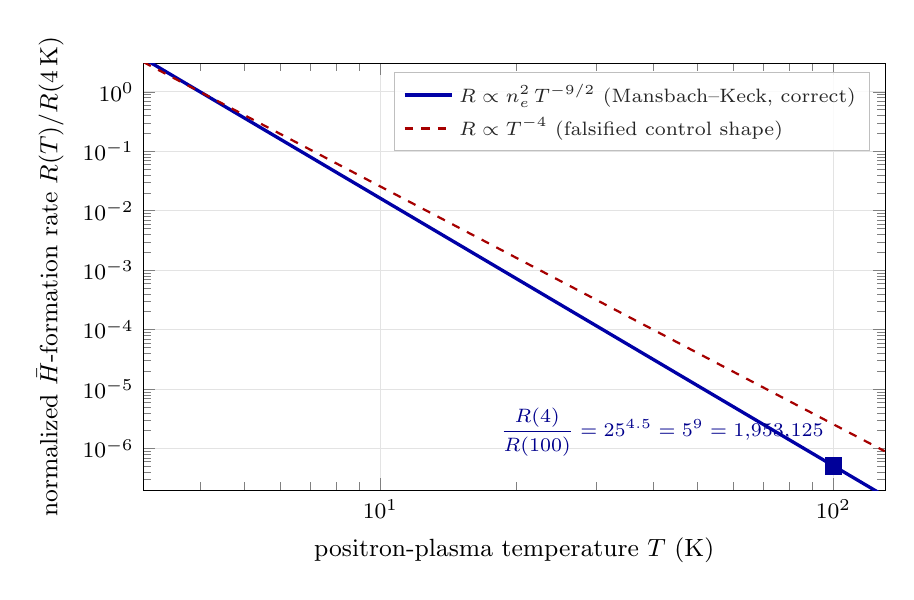
\begin{tikzpicture}
\begin{axis}[
  width=11cm, height=7cm,
  xmode=log, ymode=log,
  log basis x=10, log basis y=10,
  xlabel={positron-plasma temperature $T$ (K)},
  ylabel={normalized $\bar H$-formation rate $R(T)/R(4\,\mathrm{K})$},
  xmin=3, xmax=130,
  ymin=2e-7, ymax=3,
  tick label style={font=\footnotesize},
  label style={font=\small},
  ymajorgrids, xmajorgrids, grid style={gray!22},
  legend style={font=\scriptsize, at={(0.98,0.98)}, anchor=north east,
    fill=white, fill opacity=0.85, draw=gray!50},
  legend cell align=left,
]
% --- correct T^-9/2 scaling, normalized to T=4K ---
\addplot[blue!65!black, very thick, domain=3:130, samples=120] {(x/4)^(-4.5)};
\addlegendentry{$R\propto n_e^2\,T^{-9/2}$ (Mansbach--Keck, correct)}
% --- wrong T^-4 (falsified control implied shape) ---
\addplot[red!65!black, dashed, thick, domain=3:130, samples=120] {(x/4)^(-4.0)};
\addlegendentry{$R\propto T^{-4}$ (falsified control shape)}
% --- registered anchor: R(100K)/R(4K) = (100/4)^-4.5 = 1/1953125 = 5.12e-7 ---
\addplot[only marks, mark=square*, mark size=3pt, blue!60!black] coordinates {
  (100, 5.12e-7)
};
\node[font=\scriptsize, anchor=south east, text=blue!55!black]
  at (axis cs:100,5.12e-7) {$\dfrac{R(4)}{R(100)}=25^{4.5}=5^9=1{,}953{,}125$};
\end{axis}
\end{tikzpicture}
\end{document}
